%% Icarus submission for Encelauds paper [3rd trial, WORK IT !!]
\documentclass[preprint,12pt,3p,times,authoryear]{elsarticle}

%% Use the option review to obtain double line spacing
%% \documentclass[authoryear,preprint,review,12pt]{elsarticle}

%% Use the options 1p,twocolumn; 3p; 3p,twocolumn; 5p; or 5p,twocolumn
%% for a journal layout:
%% \documentclass[final,1p,times,authoryear]{elsarticle}
%% \documentclass[final,1p,times,twocolumn,authoryear]{elsarticle}
%% \documentclass[final,3p,times,authoryear]{elsarticle}
%% \documentclass[final,3p,times,twocolumn,authoryear]{elsarticle}
%% \documentclass[final,5p,times,authoryear]{elsarticle}
%% \documentclass[final,5p,times,twocolumn,authoryear]{elsarticle}
%
%% The amssymb package provides various useful mathematical symbols
\usepackage{amssymb}
%% The amsmath package provides various useful equation environments.
\usepackage{amsmath}
%% The amsthm package provides extended theorem environments
%% \usepackage{amsthm}

%% The lineno packages adds line numbers. Start line numbering with
%% \begin{linenumbers}, end it with \end{linenumbers}. Or switch it on
%% for the whole article with \linenumbers.
\usepackage{pifont,graphicx,amssymb,color,setspace,lineno,comment,
	booktabs,dcolumn,tabularx,pdflscape,caption,subcaption,
  longtable,dcolumn,subcaption,graphicx,lscape,caption} %,float}
%makecell,adjustbox
%\usepackage[absolute,overlay]{textpos}

\journal{ICARUS}

\begin{document}

\begin{frontmatter}

\title{The Enceladian crater production function}

\author[UniGe,ELSI]{E. W. Wong\corref{cor}}
\author[UiO]{S. C. Werner}
\author[SW]{M. R. Kirchoff}
\author[CSFK,UiO]{R. Brasser}

\affiliation[UniGe]{organization={Geneva Observatory, University of Geneva},
    addressline={Chemin Pegasi 51},
    city={Versoix},
    postcode={CH-1290},
    country={Switzerland}}

\affiliation[ELSI]{organization={Earth Life Science Institute, Tokyo Institute of Technology},
    addressline={Meguro-ku},
    city={Tokyo},
    postcode={152-8550},
    country={Japan}}

\affiliation[UiO]{organization={Centre for Planetary Habitability, Department of Geosciences, University of Oslo},
    postcode={N-0315},
    city={Oslo},
    country={Norway}}

\affiliation[SW]{organization={Southwest Research Institute},
    addressline={1050 Walnut St, Suite 300},
    city={Boulder},
    state={CO},
    country={USA}}

\affiliation[CSFK]{organization={Konkoly Observatory, HUN-REN CSFK, MTA Centre of Excellence},
    addressline={15-17 Konkoly Thege Miklos St.},
    postcode={H-1121},
    city={Budapest},
    country={Hungary}}

\cortext[cor]{Corresponding author}

%----------------------------------------------------------------------------------------------------
%
\linenumbers
%% Abstract
\begin{abstract}
Conflicting perspectives on Enceladus' past and present interior state arise from predictions of its tidal history, and an uncertain prescription of its bombardment history, as well as limited interpretation of crater statistics. Here we present the first comprehensive global crater catalogue for Enceladus and build a crater production function from our dataset. The crater production function is the underlying, unmodified crater size-frequency distribution of the satellite surface, that is, it is the pristine size-frequency distribution that the craters would have assuming no subsequent modification. We obtained the function with a data-driven approach;  therefore it makes no assumptions about the impactor source population (heliocentric versus planetocentric). The crater production function is therefore essential for computing surface ages when combined with a crater chronology function. We fit it with an 11$^{\rm th}$ degree polynomial as is customary for the Moon and Mars, indicating the waviness at different crater diameters. Future work will indicate whether the Enceladian crater production function is unique or shared with the other nearby satellites.
\end{abstract}

%%Research highlights
\begin{highlights}
\item Research highlight 1
\item Research highlight 2
\end{highlights}

%% Keywords
\begin{keyword}
%% keywords here, in the form: keyword \sep keyword

%% PACS codes here, in the form: \PACS code \sep code

%% MSC codes here, in the form: \MSC code \sep code
%% or \MSC[2008] code \sep code (2000 is the default)

\end{keyword}

\end{frontmatter}

%% Add \usepackage{lineno} before \begin{document} and uncomment
%% following line to enable line numbers
%% \linenumbers

%% main text
%%
\linenumbers
%% Use \section commands to start a section
\section{Introduction}
\label{intro}

Enceladus, one of Saturn's regular, icy satellites, displays remarkable and ongoing geyser-like cryovolcanism. Cassini’s observations, such as the south pole’s active degassing \citep{Porco2004,Spencer2006} and physical libration \citep{Thomas2016,Nimmo2023} provide strong, albeit indirect, evidence of a subsurface ocean \citep{Porco2004,Spencer2006}. Yet, the mechanisms sustaining its long-term internal activity remain unclear \citep{Nimmo2023}. Despite its small size and current low orbital eccentricity, the internal heat required to maintain this activity exceeds what is expected from tidal dissipation and radiogenic decay alone \citep{Meyer2007,Roberts2008}. Moreover, Enceladus' surface reveals a juxtaposition of both geologically young and ancient terrains.\\

In the absence of sample-return data for radiometric dating, crater counting serves as a primary tool for understanding the geological evolution of icy satellites like Enceladus. However, interpreting crater records remains challenging due to uncertainties surrounding the source, flux, and timing of impactors. Particularly for the Saturnian system, questions remain as to whether the dominant impactors are heliocentric comets or system-internal debris. While planetocentric populations may have influenced some features \citep{Ferguson2022}, the broad consensus is that heliocentric impactors, especially those originating from the scattered disc, are the primary source of cratering across the outer solar system \citep{Shoemaker1982,Chapman1986,Zahnle1998,Nesvorny2019,Wong2023,Nesvorny2023}. \\

Against this background, our study introduces two key datasets and tools. First, a new crater production function derived directly from Enceladus’ observed crater record, independent of assumed impactor population models. Second, the first global crater catalogue for Enceladus, based on a unified classification of terrain units and crater morphologies. \\

These results are crucial for advancing data-driven methods in icy satellite studies. In particular, the crater production function forms the foundational basis for future studies that aim to estimate surface ages across Enceladus. While traditional age estimates have relied on imported or theoretical crater chronologies, our production function is explicitly anchored in the observed record, enabling a more reliable, body-specific framework for later applications. \\

The detailed modelling of surface ages with an updated Enceladus-specific crater chronology will be presented in a subsequent paper. Here, we lay the groundwork by quantifying the spatial and size-frequency characteristics of craters across all major surface units, setting the stage for future geochronological interpretation.

\subsection{Terms and definitions}
\label{term&def}
In this paper, we use ``{\it crater chronology}" and ``{\it cratering}" to refer to the bombardment of the icy regular satellites, and ``{\it impact chronology}" and ``{\it impacting}" for the same processes on the giant planets. Craters form on the solid crust of the satellites whereas no long-term bombardment remnant can be preserved on the atmospheric surfaces of the giant planets. The term
``{\it size-frequency distribution}" (abbreviated to SFD) refers to a model of a statistical relationship between the diameters of craters or projectiles (interchangeable with impactors) and their frequency of occurrence, which is express as spacial density (km$^{-2}$) for craters and number of object for projectiles. A power law expression for the cumulative size-frequency distribution is $n_{\rm >D} \propto (D_0/D)^\alpha$, %$N(>D) \propto (D_0/D)^{ \alpha}$,
where $D_0$ is a scaling diameter in km, and $\alpha$ is the cumulative slope for that size ranges.
An older surface would typically have a higher crater density, which manifests as an up-shifted distribution, assuming the same source and rate of bombardment. The term ``{\it size-frequency measurement}" has the same physical nature as the {\it size-frequency distribution}; it plots the diameter of observed craters surveyed from icy satellites' images. In short, {\it size-frequency distribution} refers to a distribution that can be fitted to or derived from the observed impactor size data -- {\it size-frequency measurement}. The figures in this paper show {\it size-frequency distribution} and {\it measurement} in cumulative frequency, where the number of craters larger than a specific diameter is plotted against diameter, and the population decreases with size. \\

We usually adopt units of time of a million years and a billion years, respectively, abbreviated as ``{\it Myr}" and ``{\it Gyr}". These are counted forward in time from a particular epoch, while ``{\it Ma}" and ``{\it Ga}" mark an age, i.e., surface ages and age of the Solar System, and are generally counted backward in time from the present.

\subsection{Crater production function}
\label{sub:intro_cpf}
The crater production function (CPF) is the underlying, unmodified crater size-frequency distribution(SFD) of the satellite surface. It amounts to a calibrated crater SFD \citep{Neukum1975}, and thus enhances crater-based age-estimation techniques. Any deviation of the observed crater size-frequency distribution yields deeper insights into Enceladus’ history, in particular when specific areas were (partially) resurfaced. The CPF thus facilitates comparisons of observed crater size-frequency distributions across different regions of the same solid body, regardless of surface ages or crater density, as it is presumed to remain constant over time \citep{Neukum1975,Neukum1983,Werner2014,Werner2023}. Recent studies on the evolution of outer solar system impactor SFD also indicate that said distribution stabilised 40 Myr after planetesimal formation, and remained largely unchanged for the past 4.3 Ga \citep{Bottke2024}.\\

The choice of CPF determines the shape the age-isochrones used to estimate surface ages as crater retention ages. To our knowledge, no established CPF exists for outer Solar System satellites, so that we constructed one specifically for Enceladus, with the future aim to compute its global activity history. Previous crater studies of Enceladus have focused on specific terrains, particularly cratered plains, and inferred impactor SFDs from three main sources: Jupiter-family comets, Triton impactors, and Kuiper Belt objects \citep{Zahnle2003, Singer2019, Bottke2024}.
However, these impactor SFDs do not directly translate to crater SFDs. Moreover, they were derived from different satellite systems, where variations in planetary encounter velocities and collision velocities with the satellites affect crater formation, limiting their applicability to Enceladus and other Saturnian satellites. Finally, the published distributions mainly describe kilometre-scale impactors, with better constraints on the power-law slope for large objects (e.g., $>$10 km) than for smaller ones (e.g., $<$1 km). In contrast, observable craters on Enceladus range in diameter from a few hundred metres to 34~km. Given Enceladus’ low mass and the relatively high impact velocities of heliocentric impactors (compared to other mid-sized Saturnian satellites; \citealt{Zahnle2003, Wong2021}), most visible craters on Enceladus were formed by sub-kilometre impactors. Yet, this diameter range is where the impactor SFD becomes increasingly uncertain and inconsistent, making it unreliable for constructing a CPF. \\

\citet{Wong2023} assumed an outer Solar System-wide crater SFD derived from the SFD of Pluto-Charon craters \citep[Red line in Fig~\ref{fig:cpf_compare}]{Singer2019}. However, such a distribution does not match that of Enceladus and the other Saturnian satellites \citep[Blue line]{Kirchoff2022}). Similarly, SFDs constructed based on craters on other satellites systems, such as Ganymede, Callisto, and Europa \citep[Orange line]{Zahnle2003}, exhibit similar discrepancies \citep{Wong2023}. Consequently, no existing reference provides a reliable CPF for Enceladus, prompting the need to construct one. The SFDs used for isochron construction in \citet{Wong2023} and the CPF (in black) in this study are compared in Fig~\ref{fig:cpf_compare}.\\


\begin{figure}
    \centering
    \includegraphics[width=0.8\linewidth]{fig/compare_enc_terrains_degpoly_FigS3.png}
    \caption{Enceladus crater production function and size-frequency distributions of craters and impactors in the outer Solar System. The displayed distributions include the Enceladus crater production function derived in this study (in black), the crater size-frequency distribution fitted from the trailing hemisphere mid-latitude crater plains (\citet{Kirchoff2009}; in blue), the impactor size-frequency distribution resembling Jupiter-family comets (case A from \citet{Zahnle2003}; in orange) and collisionally evolved population (case B from \citet{Zahnle2003}; in mustard), and Kuiper belt objects (\citet{Singer2019}; in red). The dashed lines indicate diameter ranges where the distribution was not covered in the reference data but was extended with the cumulative slope of the adjacent diameter ranges.}
    \label{fig:cpf_compare}
\end{figure}
%======================================================================================================

\section{Data and Methods}
\label{sec:data}

\subsection{First global crater survey on Enceladus}
\label{subsec:crater_count}
Crater counting is a subjective process whose outcomes vary among researchers \citep{Robbins2014}. To ensure reliability, this study independently conducted crater counts on Enceladus by E. Wong (EW) and M. Kirchoff (MK). Their counts were cross-checked and combined for statistical robustness. EW surveyed craters from 50$^\circ$S to 90$^\circ$N, while MK covered from 90$^\circ$S to 60$^\circ$N, with an overlap at 50$^\circ$S to 60$^\circ$N (approximately 82\% of Enceladus' global area). During EW’s and MK’s crater counting, no lower limit was set to identify crater-like features; the minimum cutoff at 800 m for EW and 1 km for MK is applied after surveying and recording all candidate craters. For details on the crater survey and images, see Sec.~\ref{sub:survey}.\\

The combined and verified survey covered 16,958 craters using the global mosaic images from Cassini released by \citet{Bland2018}. Due to variations in (camera) emission angles, (lighting) phase angles, and image resolution among individual based images, we restrict our study to craters with diameters larger than 800 m. \\

After compiling the global crater count, we divided Enceladus into 62 geological units as displayed in  Fig.\ref{fig:division}. These divisions are based on variations in terrain geomorphology, crater distribution, and instrumental image characteristics (see App.~\ref{sub:gu} for division criteria).
Of these, 15 units, primarily on the leading hemisphere and in the south polar region, are referenced from \citet{CrowWillard2015}, while 10 units, mainly in the trailing hemisphere’s ridged plains, are adapted from \citet{Kirchoff2009}. \\

\begin{figure}[ht!]
    \centering
    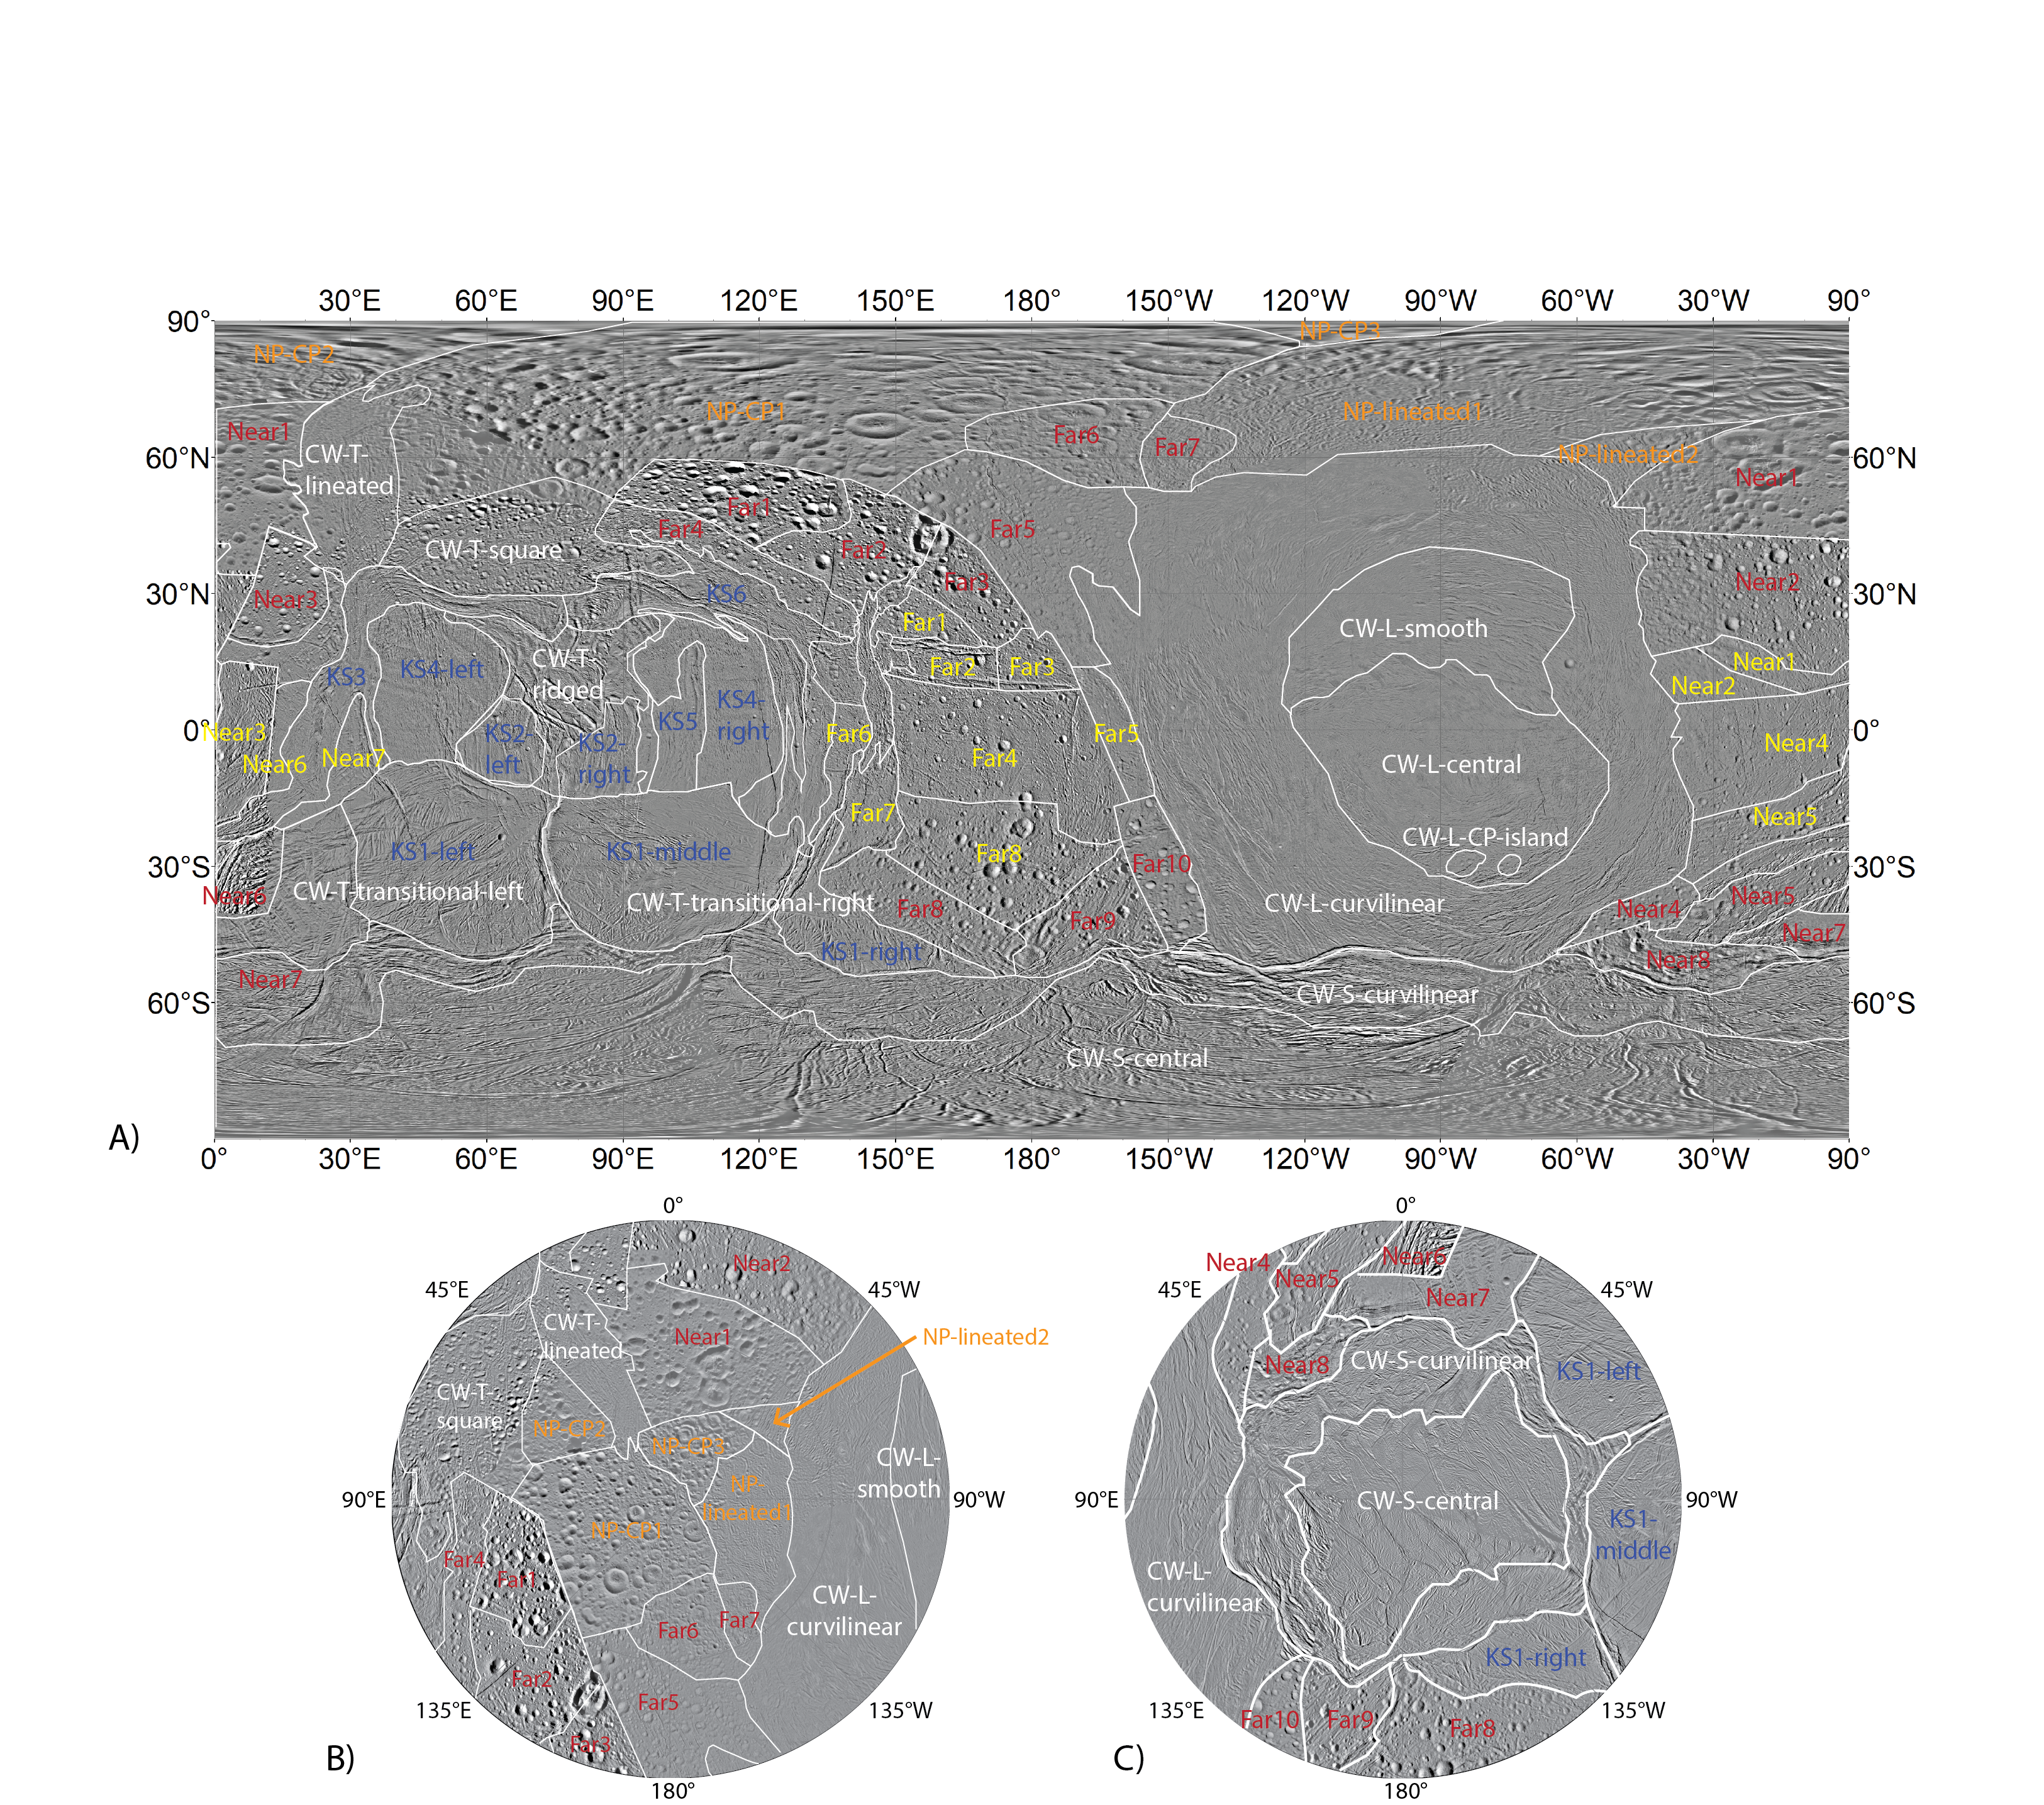
\includegraphics[width=1.0\textwidth]{fig/fig_division.png}
    \caption{Division of geologic units on Enceladus. \textbf{(A)} in equirectangular projection from  60°S to  60°N, and \textbf{(B)} and \textbf{(C)}  in polar stereographic from pole to 30° latitude in the north and south poles, respectively. Due to space constraints, not all units are labelled with full names. The prefix “RP” for ridged plains from \citet{Kirchoff2009} is omitted. Colour variations (red and yellow) distinguish between “Mid” (for mid-latitude) and “Eq” (for equator) without repeated labelling. Units in the north pole defined in this work are labelled in orange. Units referencing \citet{Kirchoff2009} are in blue, while those referencing \citet{CrowWillard2015} are in white. }
    \label{fig:division}
\end{figure}
%------------------------------------------------------------------------------------------------------

\subsection{Preparing crater counts to construct the Enceladus-specific crater production function}
\label{subsec:cpf}
Tectonic activities are hypothesised to selectively remove smaller craters while leaving larger ones relatively intact \citep{Michael2010}. Consequently, the observed crater size-frequency distribution (SFD) gradually, and possibly irregularly, rolls off towards the smaller end, leading to two distinct ages when fitting for surface ages within different diameter ranges. Ages modelled by including smaller craters will appear younger than those relying solely on large craters. As such, for correct age estimation we need the crater production function (CPF).\\

After acquiring the global crater database, we analysed it alongside surface morphology to assess how tectonic resurfacing alters the crater SFD. In particular, we examined craters with diameters comparable to the size of tectonic features that traverse the same terrain or those susceptible to be removed by partial resurfacing, often extending from adjacent, younger terrains. This analysis allowed us to identify the minimum crater diameter that remains largely unaffected by geological activity, which varies by region, typically from 1~km to 5~km. In heavily cratered regions, small craters are preferentially erased by subsequent impacts, flattening the slope at the small end of the SFD. In tectonically active areas, ridges and troughs obscure or erase craters of similar length scale. Conversely, in smoother, recently resurfaced terrains, newly formed smaller craters could be distinguishable, with some preserved down to 1~km. Establishing this threshold diameter enables the construction of an initial, non-geologically modified crater SFD, which serves as a basis for the CPF.\\

\begin{figure}[ht!]
    \centering
    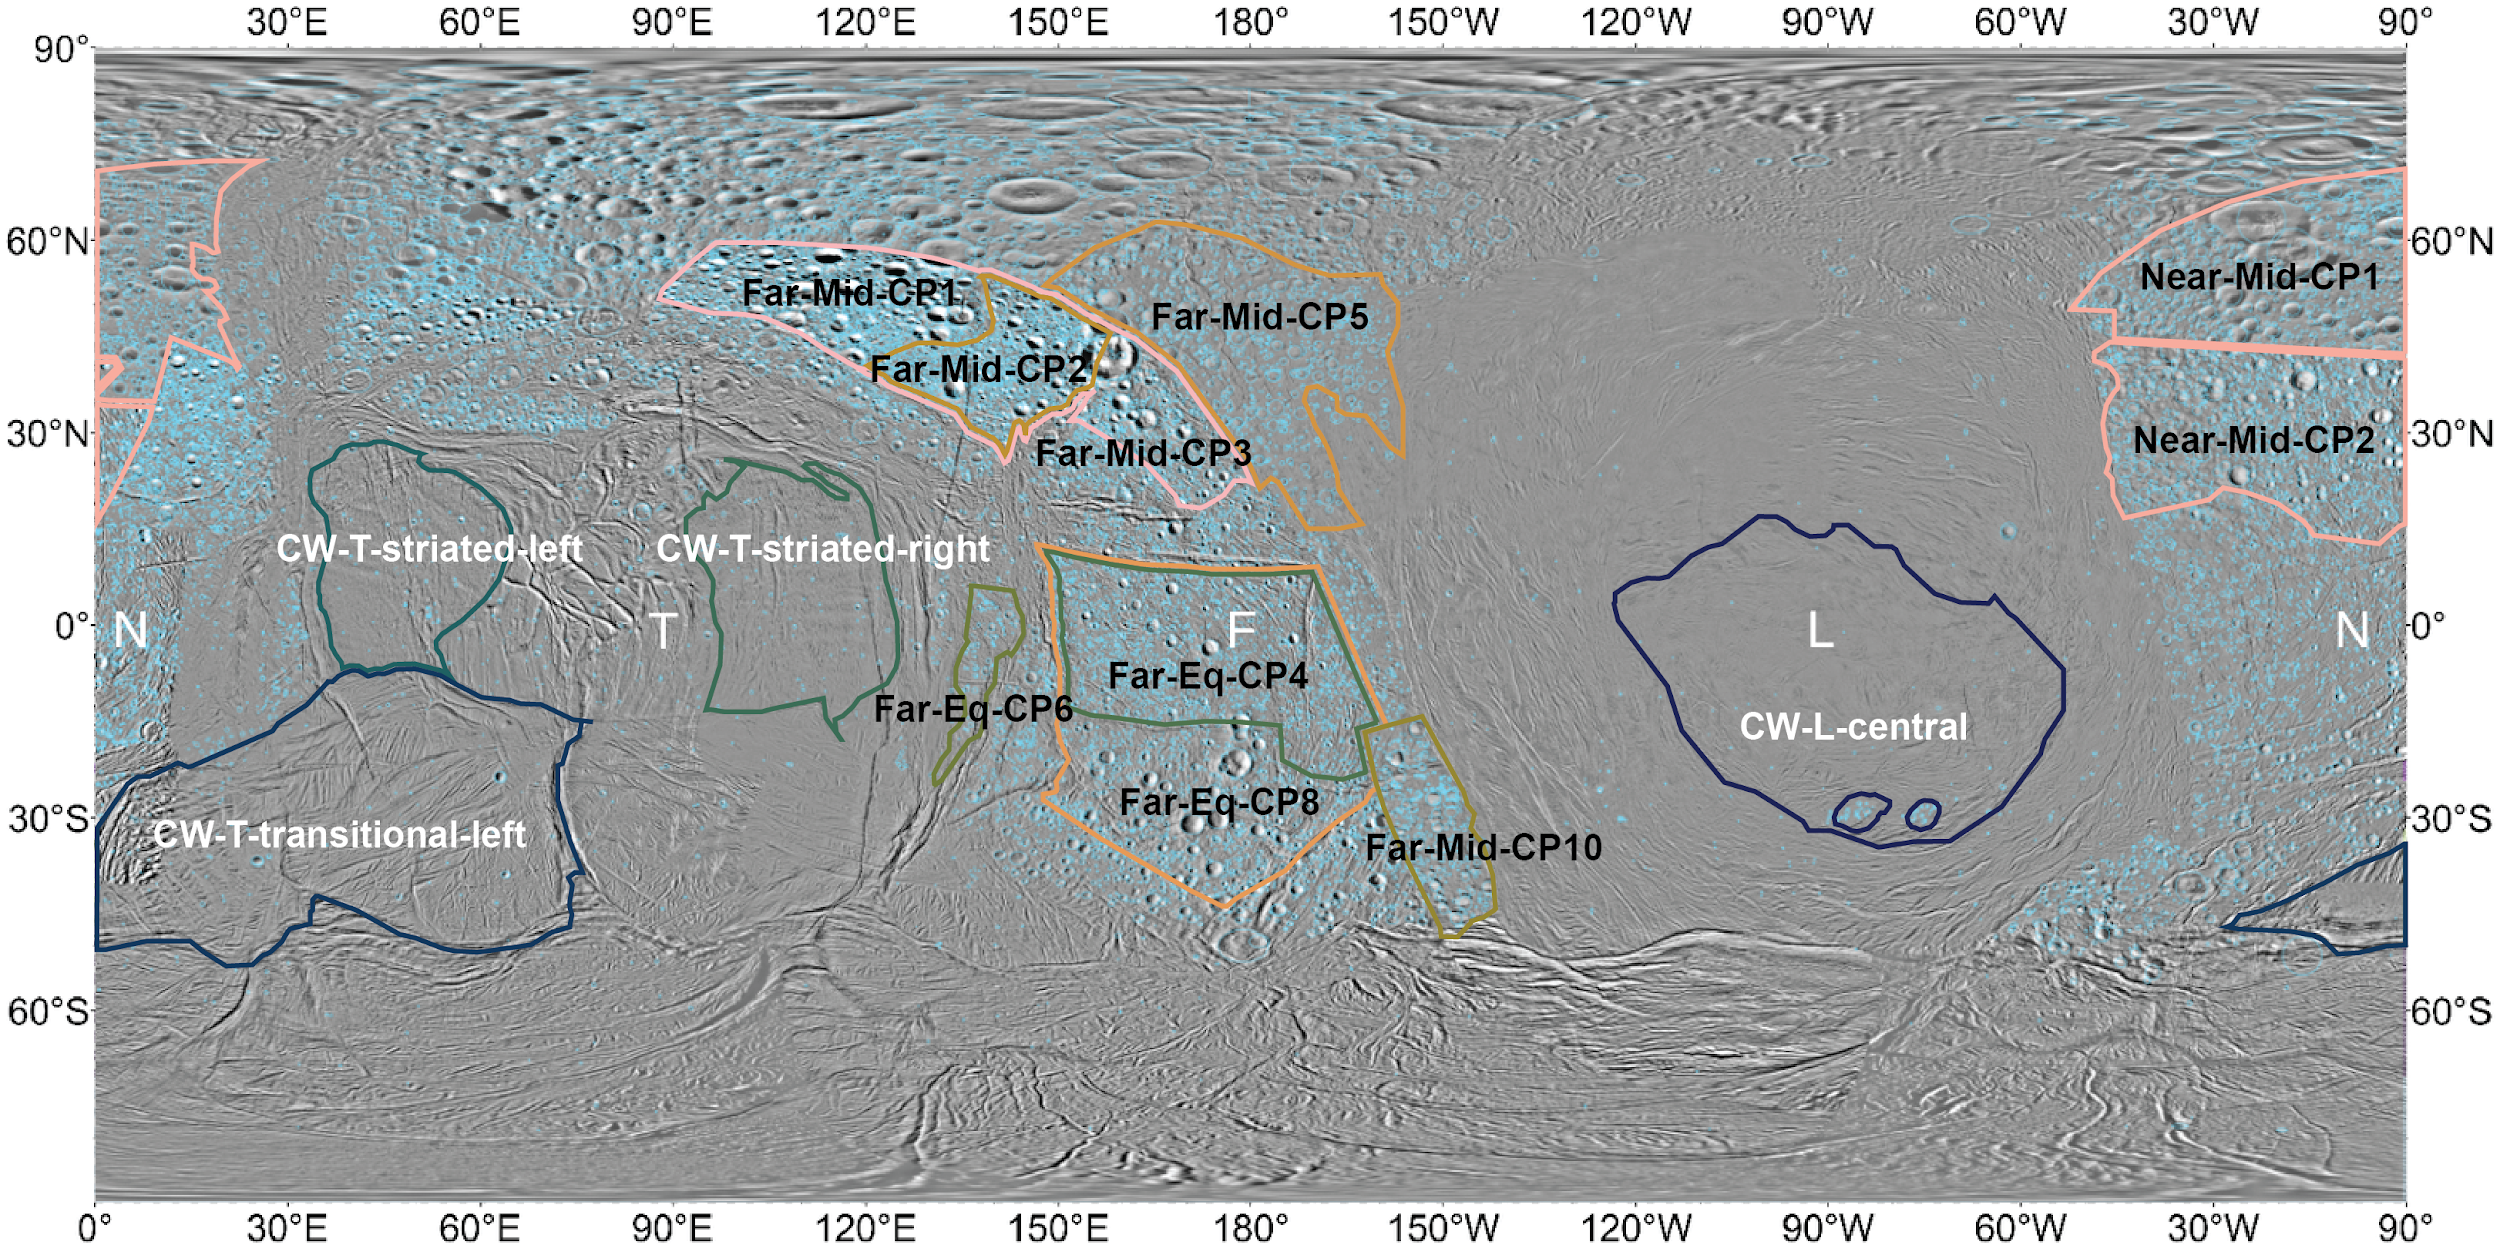
\includegraphics[width=0.8\textwidth]{fig/fig1a.png}
    \includegraphics[width=0.3\textwidth]{fig/fig1b.png}
    \includegraphics[width=0.3\textwidth]{fig/fig1_arrow.png}
    \includegraphics[width=0.3\textwidth]{fig/fig1c_with_model.png}
    \caption{Construction of the crater production function (CPF).
        \textbf{(A)} Representative geological units overlaid on global mosaic images of Enceladus. White names denote units referenced from Kirchoff \& Schenk (2017) and Crow-Willard \& Pappalardo (2018), while black names denote units defined in this study.
        \textbf{(B)} Crater size-frequency measurements for each unit with logarithmic binning at 0.05 intervals. Transitioning colours (navy to pink) indicate increasing crater density and larger typical diameters. The error bars represent Poisson errors.
        \textbf{(C)} Visualisation of the upscaling and alignment of the crater measurements.
        \textbf{(D)} Normalised size-frequency measurements relative to the crater density of Far-Mid-CP5, with the black line shows a 10$^{\rm th}$-degree polynomial fit for the CPF.
        \textbf{Emi: will align the Fig B, C, \& D on the same height at the end}}
    \label{fig:age}
\end{figure}

%To correctly interpret Enceladus’ resurfacing history, we require the CPF, which
We constructed the CPF from craters 800 m to 35 km in diameter, encompassing the minimum resolvable diameter to the maximum one. To explore the entire range, we selected 13 representative geologic units for different diameter categories (see Fig.\ref{fig:age}A). For the smaller craters ($<$3 km), we focused on sparsely cratered smooth plains devoid of large impacts to minimise the risk of removal or contamination by secondary craters. For rarer large craters ($>$10 km), we utilised measurements from heavily cratered terrains, where more craters have accumulated, to ensure statistical accuracy across expansive areas.\\
 %We selected terrains or geological units defined by \citet{Kirchoff2009}, \citet{CrowWillard2015}, and from this work (see Fig. S1).
 %Table S1 offers numerical specifics of representative geologic units, crater counts, and diameter ranges for CPF modelling. \\

\begin{table}[t]
\centering
    \begin{tabular}{p{4.0cm} p{3.0cm} p{2.0cm} p{3.0cm}}
\hline
\textbf{Geologic Unit} & \textbf{Lat., Long. (°)} & \textbf{No. Craters} & \textbf{Fitting Diameter Range (km)} \\
\hline
CW-L-central & 90°W, 10°S & 34 & 0.8$\sim$1.5 \\
CW-T-transitional-left & 35°E, 30°S & 125 & 0.9$\sim$2.5 \\
CW-T-striated-left & 50°E, 10°N & 86 & 0.8$\sim$2.2 \\
CW-T-striated-right & 110°E, 5°N & 120 & 0.9$\sim$2.5 \\
Far-Eq-CP4 & 175°E, 30°S & 1576 & 1.5$\sim$14 \\
Far-Eq-CP6 & 137°E, 10°S & 125 & 2.0$\sim$5.0 \\
Far-Mid-CP3 & 166°W, 30°N & 436 & 3.5$\sim$32 \\
Near-Mid-CP2 & 18°E, 14°N & 1450 & 5.0$\sim$15 \\
Far-Mid-CP10 & 152°W, 30°S & 338 & 3.0$\sim$7.0 \\
Far-Mid-CP5 & 180°W, 40°N & 813 & 4.0$\sim$10 \\
Far-Mid-CP2 & 142°W, 42°N & 579 & 3.2$\sim$32 \\
Far-Eq-CP8 & 175°E, 30°S & 857 & 4.3$\sim$21 \\
Far-Mid-CP1 & 115°W, 50°N & 638 & 4.0$\sim$16 \\
Near-Mid-CP1 & 32°E, 12°N & 1138 & 4.0$\sim$35 \\
\hline
\end{tabular}
\caption{List of the representative geologic units used to derive the crater production function. From left to right are the name codes, rough coordinates of the centre of the unit, number of crater counted within the unit, and the crater diameter ranges (in km) used to fit and scale for the crater production function. The ages are in billion years old (Ga) unless specified in million years old (Ma).}
\label{tab:craters}
\end{table}

In Figure~\ref{fig:age}B, we illustrate the observed size-frequency measurements of the 13 representative geologic unit (as listed in Table~\ref{tab:craters}). The measurements are plotted, binned logarithmically in crater diameter with a width of 0.05.
Some units exhibit a large amounts of craters spanning a wider diameter ranges, while certain smaller units are combined for a broader search area and larger statistical base to derive the function at larger crater ranges. To enhance statistics, ideally all diameter ranges should be represented by several measurements from various units. However, measurements are based on regions with different image resolutions, degrees of resurfacing, and post-impact modifications, allowing only a limited accurate or representative crater size range (see Fig. 12 of \citealt{Bland2018}). Therefore, we considered the largest possible overlap of individual measurements to minimise statistical uncertainties and avoid gaps. The arrows indicate the next step: aligning the data.\\

Figure~\ref{fig:age}C showcases the same data as in Fig.~\ref{fig:age}B, with the arrows indicating by how much the crater density for small crater diameter has to be increased to align with the crater density profile at large crater diameters. The resulting CPF's profile when all crater measurements are aligned against a reference crater distribution is shown in Figure~\ref{fig:age}D. We chose the ``Far-Mid-CP5'' terrain for its broad range of crater diameters and intermediate crater density. To normalise the measurements of the other 12 representative geological units, we determined the vertical scaling factor by averaging the ratio of crater frequencies within the diameter range where the crater measurements overlap and show the best agreement. This approach follows the methodology used for the lunar CPFs, both in the historical work of \citet{Neukum1975} and the recent study by \citet{Xiao2024}. Once aligned, the crater size-frequency measurements from the representative geologic units with different crater densities were standardised and combined, forming a representative set of SFDs to trace the CPF (Fig.~\ref{fig:age}D).\\

\subsection{Fitting of the crater production function}
\label{subsec:fitting}
The crater production for Mercury \citep{Neukum2001}, Mars \citep{Ivanov2001, Hartmann2005}, and asteroids: Vesta, Ida \citep{Schmedemann2014}, and Ceres \citep{Hiesinger2016} have been derived by fitting a mathematical function to the normalised crater SFDs, such as polynomials or piecewise power laws. The former has traditionally been used for the lunar CPF (e.g., \citealt{Neukum2001}), while the latter is more common for describing impactor distributions in the outer Solar System (e.g., \citealt{Zahnle2003}). These empirical functions enable the translation of crater densities across different size ranges. \\

For Enceladus, we determined that a 11$^{\rm th}$-degree polynomial best represents the CPF for craters between 800~m and 35~km in diameter, preserving a continuous downward slope in the distribution (Fig.~\ref{fig:age}D). The polynomial fit is given by:
\begin{equation}
    \log N_{D_{\rm cr}} = \sum_{i=0}^{j} a_{i} [\log D_{\rm cr}]^i,
    \label{equ:cpf}
\end{equation}
where $N_{(D_{\rm cr})}$ is the cumulative crater frequency, $D_{\rm cr}$ is crater diameter in km, and $j = 10$ and log is the logarithm of base ten. Table~\ref{tab:cpf} presents the polynomial coefficients from $a_{0}$ to $a_{10}$.\\
%;or in an expanded form:
%\[ \log_{10}(N_{(D_{\rm cr})}) = a_{0} + a_{1}\log_{10}(D_{\rm cr}) + a_{2}\log_{10}(D_{\rm cr})^2 + ... + a_{10}\log_{10}(D_{\rm cr})^{10}. \]
\begin{table}[t]%% placement specifier
\centering
\begin{tabular}{cc}
\hline
\textbf{n (degree)} & \textbf{$a_n$} \\
\hline
0 & 6.3077  \\
1 & -2.3503 \\
2 & -5.5573 \\
3 & 24.951  \\
4 & -77.268 \\
5 & 212.99  \\
6 & -406.68 \\
7 & 464.58  \\
8 & -303.37 \\
9 & 104.74  \\
10 & -14.850 \\
\hline
\end{tabular}
\caption{Coefficients of the Enceladus’ crater production function as 11$^{\rm th}$ degree polynomials.}
\label{tab:cpf}
\end{table}

To facilitate comparison to a piecewise linear power-law fitting, where different crater diameter ranges follow distinct power-law slopes, we note that the corresponding cumulative power-law slope of this polynomial varies from -2.6 to -4.2. It is shallower below a crater diameter of 3 km and steeper beyond 7 km in crater diameter. However, these changes are not intense enough to indicate a break in the SFD at a crater diameter of 7--8 km. Such steepening at larger diameters may be attributable to the edge effect of the rarity of large craters. A previous study reported similar slopes, ranging from -1.4 to -2.9 for smaller craters, and -3.0 to -4.3 for craters larger than 7 km (\citealt{Kirchoff2009}, Table 2). The slopes derived from our CPF neatly fall within previous literature ranges.\\

We end with the following statement: the CPF does not assume whether impactors are heliocentric or planetocentric in origin or their relative contributions, as the CPF construction is data-derived from crater counts rather than model-based predictions.

%Deviations in crater size-frequency measurements away from the isochrones indicate surface modifications by endogenic (e.g., tectonic activity) or exogenic (e.g., infalling E-ring material deposition) processes; similar principles (but different mechanisms) have been proposed for lunar crater studies \citep{Neukum1975}.

%Finally, since the CPF is assumed to remain constant over time, we scaled it vertically in the cumulative SFD plot, using the expected crater density from Enceladus' modelled crater chronology (Sec.~\ref{sub:cc}) to construct age-isochrones.
%This allowed us to model the expected crater densities across different ages and crater sizes (Fig.~\ref{fig:age}F). Most importantly, by comparing observed crater size-frequency measurements with these isochrones (Fig.~\ref{fig:age}G), we determined the best-fit ages for each terrain.
%Finally, assuming that cratering is dominated by a time-invariant impactor population with a static SFD , an assumption also applied to the inner solar system \citep{Neukum1975,Neukum1983},we combined CPF and chronology to construct age-isochrones which provide the expected crater densities across different ages and crater size (Fig.~\ref{fig:age}F). The isochrones are fitted directly to the observed crater size-frequency measurements to determined the best-fit surface ages for each terrain (Fig.~\ref{fig:age}G).

\subsection{Details of crater survey}
\label{sub:survey}
EW’s survey utilised the geodetically controlled global mosaic images released by \citet{Bland2018}, comprising 108 high-resolution images (55 to 419 m/pixel), with 96\% of the total area below 200 m/pixel resolution, and 18\% below 100 m/pixel. Despite this, visual variations affect the minimum resolvable crater diameter instrumentally. For instance, sub-kilometre craters are visible in mid-latitudes and equatorial regions, but are challenging to discern around the north pole due to lower resolution, despite expectations of similar crater abundance based on the crater count at large diameter ranges and the region’s proximity. Furthermore, the solar incidence angle can affect crater identification \citep{Ostrach2011}. One of the primary regions affected by this is the central leading hemisphere, where the low incidence angles reduce crater visibility.\\

MK's counts have been gathered for over a decade (2007–current) and have used the greyscale mosaics generated by Paul Schenk throughout that time frame \citep{Schenk2011,Schenk2018} with the most recent being published in \citet{Schenk2024}. Measurements were updated and added in both location and diameter as cartography and imaging improved \citet{Kirchoff2016,Kirchoff2018}. As the images used in the mosaic did not vastly differ from those used by \citet{Bland2018}, similar issues affected MK's counts as EW's counts discussed above.\\

EW employed ArcGIS with the CraterTools add-in \citep{Kneissl2011} and QGIS with the OpenCraterTool add-in \citep{Heyer2023} to locate and document the diameter and coordinates of candidate craters. MK employed both USGS ISIS (for only the earliest counts; \citealt{Kirchoff2009}) and JMARS (http://jmars.asu.edu/; \citealt{Christensen2009}) to measure crater diameters and locations.  In JMARS both the 3-point crater counting and ellipse shape tools were used.

\subsection{Division of geological units}
\label{sub:gu}
This study’s geologic unit divisions reference two earlier works: the global geomorphology studies by \citet{CrowWillard2015}, and crater distribution studies focusing on the trailing hemisphere by \citet{Kirchoff2009}. Previous divisions have broadly treated certain regions as a single unit. For instance, \citet{CrowWillard2015} considers 320,000 km$^{2}$, or 41\% of Enceladus, as a massive cratered plain. Even though \citet{Kirchoff2009} separated the anti-Saturn side cratered plains into mid-latitude and equatorial cratered plains, both span wide areas and apparent differences exist within these expansive cratered plains. Moreover, cratered plains on the Saturn-facing side hemisphere have yet to be extensively studied. Combining surfaces with potentially varied solidification time and geological histories, especially a younger surface with a lower crater density, dilutes the crater count, resulting in a turnover or reduced slope in the SFD of small diameter ranges. This leads to inaccurate fitting of surface ages. \\

To ensure representative crater count and size-frequency measurements, vital for deciphering surface ages and regional geological history, we divided Enceladus’ entire surface into 62 geologic units based on three criteria of difference: geomorphology, crater distribution, and instrumental image characteristics.

\subsubsection{First criterion: geomorphology}
Craters, being circular or elliptical, stand out prominently from most tectonic features, such as ridges, troughs, and chasmata, which are often linear and parallel. However, challenges arise in distinguishing craters from tectonic features of similar scales, particularly when the width of curvilinear troughs, as seen in the transitional units (CW-T-transitional-left/right) defined by \citet{CrowWillard2015}, resembles that of small craters (1 to 3.5 km wide). The cross-cutting troughs may produce quadrilateral or circular-like features that mimic small craters. In cratered plains, heavily eroded ``squarish" craters and craters intersected by pit chains can be challenging to discern and measure. The size and shape of these questionable craters vary across geologic units due to differences in background topography, requiring separate consideration of crater counts from each unit.\\

Ridges and troughs abound on Enceladus’ younger surface form in large groups with similar widths and run almost parallel, dominating specific regions such as the anti-Saturn side southern mid-latitude cratered plain (Far-Eq-CP3) and the trailing hemisphere transitional plain (KS-RP1-middle). Identical ridge or trough groups within a geologic unit suggest resurfacing by the same event, implying identical surface ages and crater densities. Nevertheless, units with similar morphology might form at distinct times through a similar process. Therefore, it is essential to consider the superimposed crater population as a criterion to distinguish units that may appear similar, but have formed at different times.

\subsubsection{Second criterion: observable general crater distribution}
Crater density evidently varies across regions, even within the cratered plains and subdued cratered plains by \citet{CrowWillard2015}. Calculating surface ages relies heavily on crater density, as older surfaces accumulate more craters. Mixing crater counts from geologic units that solidified at different times skews the average crater density and misrepresents solidification ages. Accurate age calculations necessitate bounding geologic units to areas with similar crater densities. However, Enceladus poses specific challenges due to its complex and multiple resurfacing events because not all surfaces underwent full resurfacing, where the entire crust melted and resolidified, erasing all pre-existing features, including craters, and resetting ages. Instead, surfaces might be partially resurfaced. Some cratered plains display a gradual decrease in crater density, such as from high to low latitudes, or as surfaces approach the boundaries of crater terrains or specific tectonic features. Overall, changes in crater density indicate variations in underlying surface ages, necessitating the classification of distinct geologic units.\\

Manually drawing units’ boundaries based on cumulative crater density could be arbitrary. Although different studies define boundaries differently based on visually prominent surface morphologies, subdivision based on crater density as additional criterion avoids unrepresentative crater count interpretations and improves age estimation.

\subsubsection{Third criterion: instrumental image characteristics}
Variations in the surface images of Enceladus affect crater counts and geomorphology identification. Image resolution limits the minimal recoverable crater diameters and can artificially flatten the size-frequency measurement as crater diameters approach the resolution limit. If a geologic unit spans images with different resolutions, there will be a drop in the smaller crater count in part of the unit, creating an illusionary flattening in the size-frequency measurement. To mitigate this, it is safer to separate such units.\\

Solar incidence angle — the angle between the incoming light direction and the surface perpendicular line — influences shadow length and visibility. Higher incidence angles result in longer, more pronounced shadows, revealing details such as crater wall shadows.
Lower incidence angles, typical at noon, produce uniform illumination, making it difficult to discern surface irregularities and small-scale topography like relaxed craters and linear ridges/troughs with slighter elevation changes. Emission angle is the angle between Cassini's camera viewing direction and the surface perpendicular line. At high emission angles, features become distorted and size measurement accuracy (e.g., width of ridges/trough and crater size) may be inaccurate. For visual examples of appearance changes due to different incidence and emission angles, refer to Fig. 2 in \citet{Bland2018}.\\

Variations in imaging conditions inherently yield diverse observed crater density and size-frequency measurements. Combining crater counts across images may render crater density and size-frequency measurements unrepresentative of the actual surface ages and geological history.\\

Shown in Fig~{\ref{fig:division}, Enceladus is divided into 62 geologic units. Those that have been designated by \citet{CrowWillard2015} are prefaced with ``CW'', those by \citet{Kirchoff2009} with ``KS'', and followed by location indicators: ``T'' for trailing hemisphere, or ``L" for leading hemisphere. The newly defined units in this work, mostly the cratered plains, are prefaced with ``Far'' and ``Near'' to denote their locations on Enceladus' Saturn-facing and anti-Saturn sides, respectively, followed by ``Mid'' for mid-latitude or ``Eq’ for equatorial region. North polar regions are prefaced with ``NP'' followed by ``CP'' or ``lineated'' for crater plains and lineated plain, respectively. For the south polar region, we follow those previously defined by \citet{CrowWillard2015}, thus the south polar curvilinear plains (CW-S-curvilinear) and central plain (CW-S-central). \\
\textbf{Shall we still list all the geolgical unit, their full name and rought central coordinate and number of crater counted, could also share something like the maxiumum crater counted on that unit.}}
%Please consult Table S2 for a comprehensive list of each geologic unit’s name code.\\
Here we like to remind the reader that, while a geologic unit typically denotes a distinct surface area with similar formation, composition, age, and geological history, the term ``geologic unit'' in this study may not precisely adhere to this definition due to its division based on image disparities, in addition to geomorphology and crater distribution. Consequently, two units in this study may be combined. Readers should regard the ``geologic unit" in this work, especially those subdivided in cratered plains, as a ``potential geological unit".

%------------------------------------------------------------------------------------------------------

\section{Results}

\subsection{Global crater distribution}
\label{subsec:crater_dist}

\begin{figure}[ht!]
    \centering
    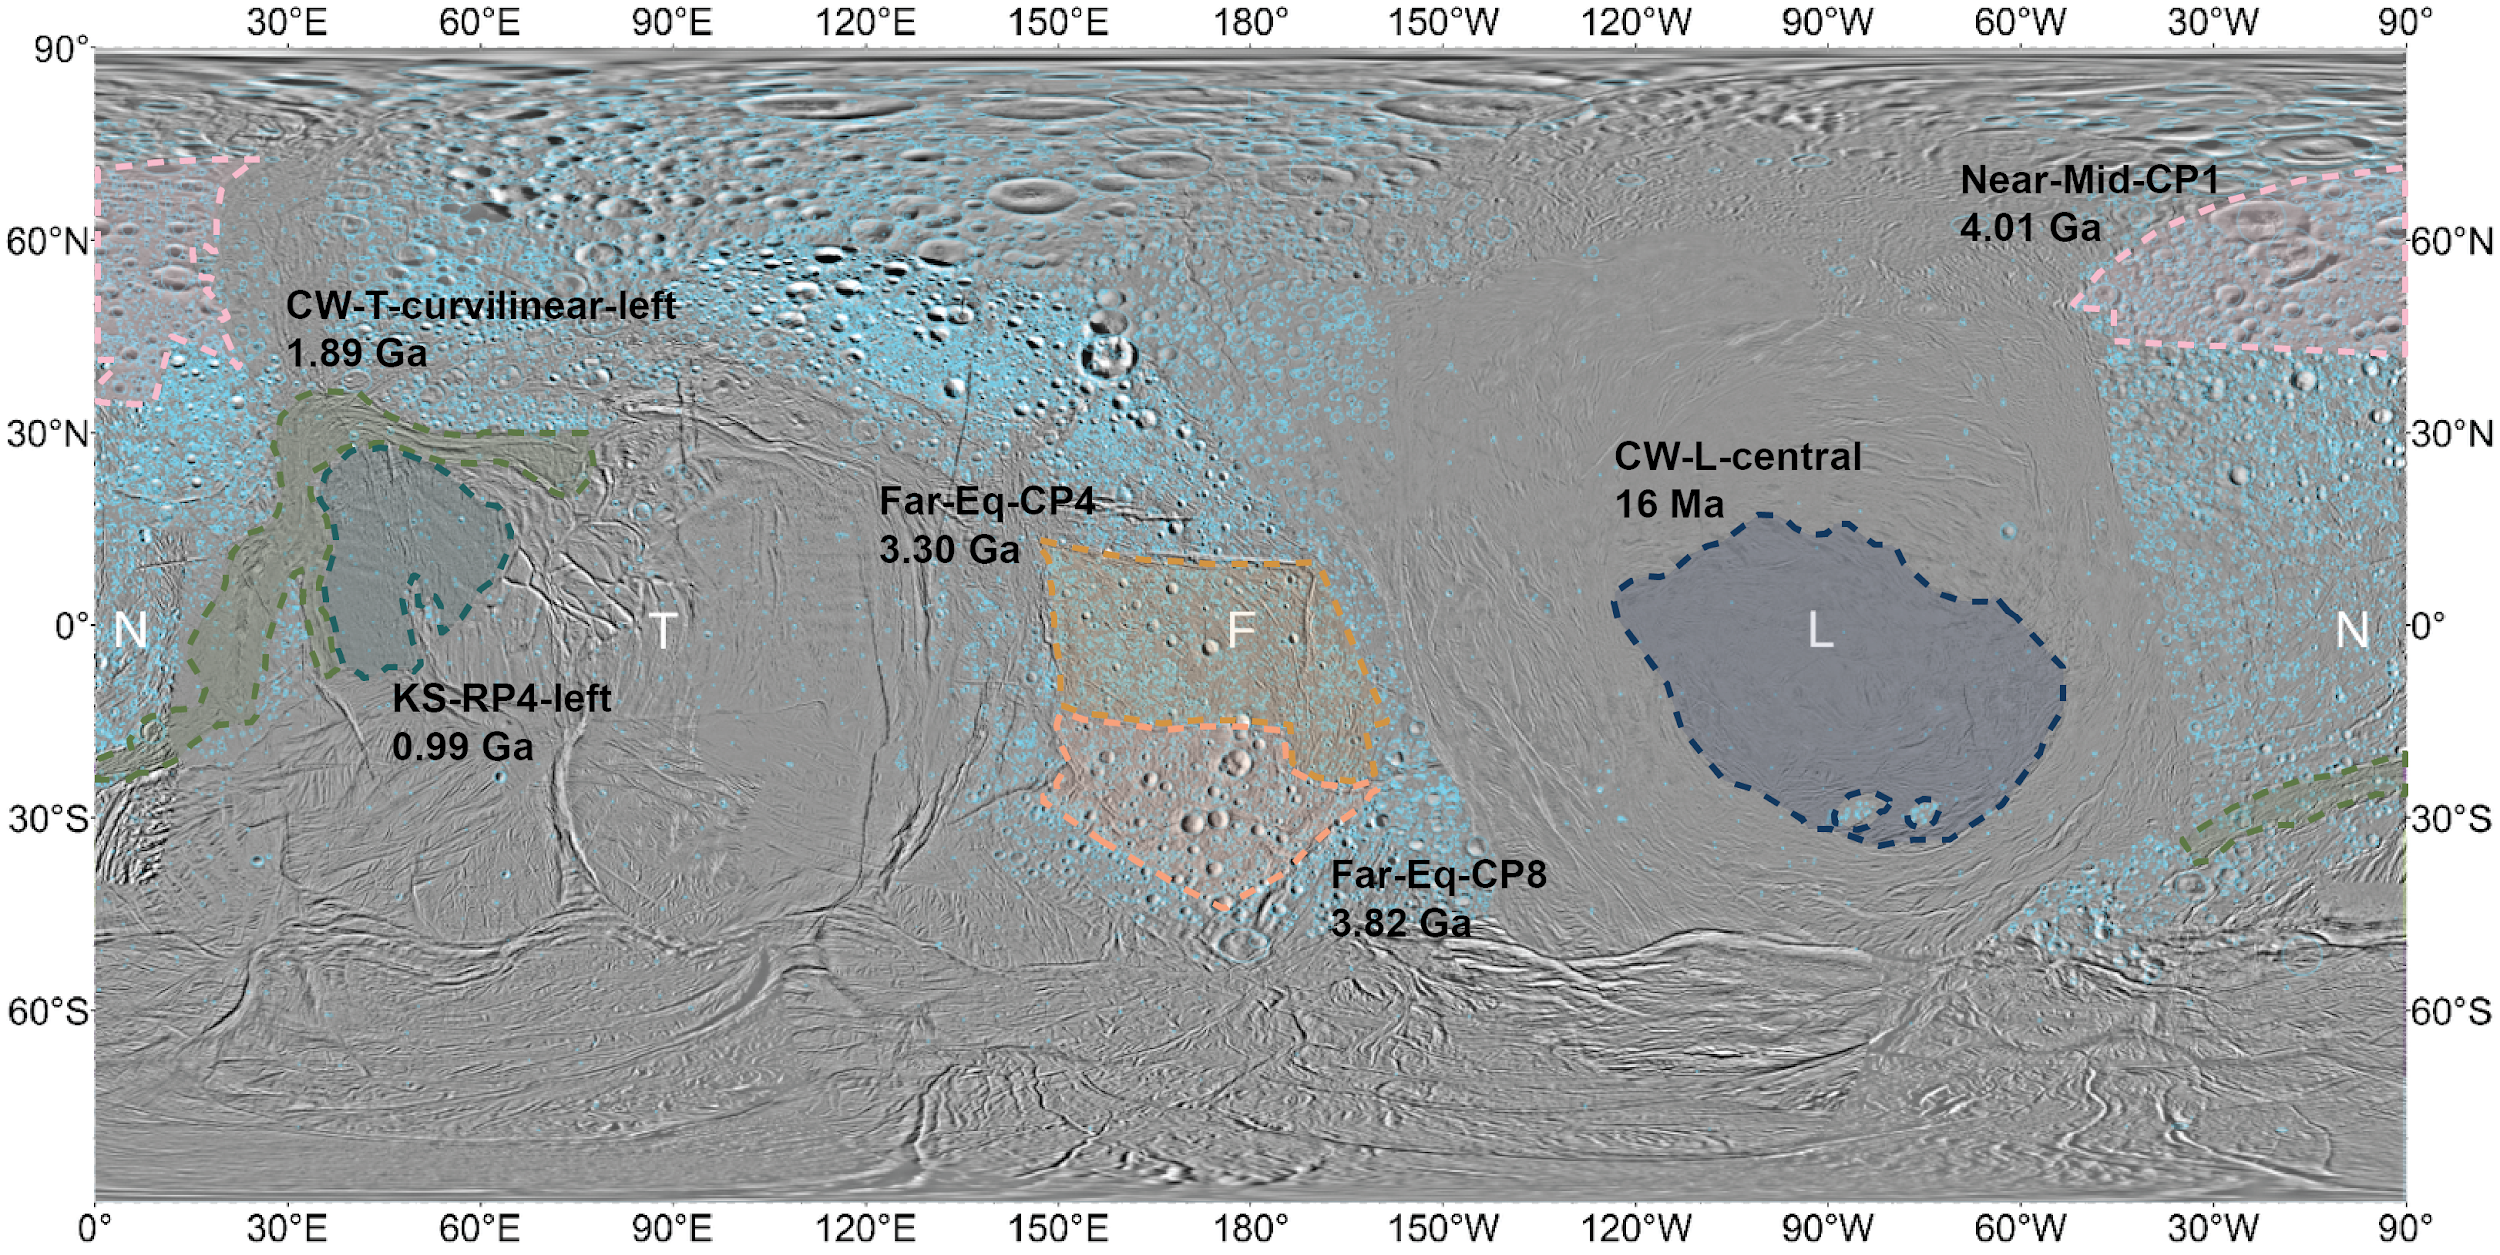
\includegraphics[width=0.8\linewidth]{fig/fig4a_plotted_GU.png}
    \includegraphics[width=0.5\linewidth]{fig/compare_fig4_icarus.png}
    \caption{Demonstration of different crater populations across six geological units.
        \textbf{(A)} Cyan elliptical outlines highlight the uneven distribution of craters across Enceladus. Thin dashed lines bounding the semi-transparent areas mark the six distinctive geological units, each labelled with its name and best-fitted crater retention ages. Capital letters along the equator (N, T, F, L) represent the Near-side, Trailing, Far-side, and Leading hemispheres, aiding in unit location reference.
        \textbf{(B)} Raw and unbinned crater size-frequency measurements in cumulative distribution for the six geological units, with colours matching those in (A). Error bars represent Poisson errors. These measurements are compared with age-isochrones reflecting crater size-frequency distributions at modelled surface ages from 1 Ma to 4.4 Ga. Differences in slope reflect variations in surface age, location, and resurfacing degree. The six units were chosen to minimise resurfacing effects that obscure slopes. }
    \label{fig:crater}
\end{figure}

Enceladus' craters are heterogeneously distributed across its icy surface. As depicted in Figure~\ref{fig:crater}A, the northern high latitude region (beyond 40$^\circ$N) and in longitudinal direction narrow regions along the Saturn-facing side (~0$^\circ$) and anti-Saturn side (~180$^\circ$) are densely cratered. Additionally, clusters of craters, such as those around 80$^\circ$W, 30$^\circ$S; and 30$^\circ$E, 0$^\circ$, are observed within the more expansive yet scarcely cratered leading and trailing hemispheres. The heterogeneity in the crater distribution is attributed to regional resurfacing of the icy crust, which has erased previous impact records, rather than being caused by preferential impact at specific locations on the satellite, i.e. the apex-antapex impact asymmetry (e.g. \citealt{Cuk2016}). For further discussion on crater heterogeneity, see Section~\ref{sub:hetero}.\\

Figure~\ref{fig:crater}B compares the observed crater SFD across different geologic units on Enceladus. Each unit has a SFD that is an approximate power law. The SFD slope changes from one unit to another. Among the less densely cratered units (green and blue curves) the slopes are very similar. Conversely, the two SFDs for the most densely cratered units (orange and pink) differ from each other and exhibit a gradual decrease (roll-off) at distinct diameters (around 3$\sim$4 km).\\

One could argue this rolling-off results from a change in the cratering population with time. Yet, geomorphological analysis points towards partial resurfacing as a plausible and more straightforward explanation, selectively removing small craters first, and most prominently for the old cratered plains \citep{Michael2010}. Newly formed craters suffered less erosion from ongoing tectonic and other resurfacing activities. Cassini’s images reveal ample evidence of partially eroded or traversed craters within the ancient cratered plains, affected by tectonic structures extending from neighbouring, younger surfaces. (see Appendix)\\

In Figure~\ref{fig:age}B, we illustrate the observed raw size-frequency measurements of the representative geologic unit (as listed in Table~\ref{tab:craters}). Each SFD is computed by binning the number of craters in logarithmic intervals of 0.05. %; isochrones serving as age references are also shown, and are calculated from both our updated crater chronology and the new CPF from this study; the shown isochrones are thus modified from those in \citet{Wong2023}.
Figure~\ref{fig:age}D showcases the resulting CPF when all measurements are normalised, building on the reference unit ``Far-Mid-CP5'' (selected for its wide-ranging diameter scales and intermediate surface ages). The CPF takes the normalised crater SFDs and combines them into a single SFD, which we fitted with a polynomial following \citet{Neukum2001}. \\

%Figure~\ref{fig:age}D and Figure~\ref{fig:crater}B show that Enceladus has undergone continuous or episodic resurfacing (or has been internally active) for the last 4 Gyr. The distribution of absolute surface ages can be categorised into six key regions, ranging from the oldest to the youngest, which is still active: the north pole, mid-latitude region, equator, central trailing hemisphere, central leading hemisphere and south pole. The crater retention ages depict the modelled age and time since which the solidified surface endured impacts and retained craters up to the present day. (See Table S2 for the best-fit initial solidification ages and resurfacing ages for each geologic unit defined in this work).

%=====================================================================================================

\section{Discussion}

%\subsection{Crater relaxation}
%\label{subsec:relax}
Recently \citet{Bland2012,Martin2023} indicate that Enceladus’ low gravity, current heat flux of $<$40 to $>$120 mW m$^{-2}$ \citep{Cadek2019,Kinczyk2024}, and surface temperature of $\sim$70 K make complete crater burial through viscous relaxation and burial by south polar plumes and E-ring material alone unlikely. However, the observed crater relaxation (e.g., \citealt{Bland2012}) and scarcity of large craters near the equator likely required a short period of excessive heat flux ($>$150 mW m$^{-2}$) and warmer subsurface temperatures ($\sim$150 K). Such condition, possibly enhanced by insulation from regolith or plume material. Under a constant heat flux of 150 mW m$^{-2}$ on a 150 K surface, craters 15–20 km in diameter with depth-to-diameter ratios of $\sim$0.2 could relax by over 80\%. Moreover, at a current maximum equatorial deposition rate of $\sim$10$^{-3}$ mm yr$^{-1}$, these craters could be buried within few hundred million years \citep{Bland2012}. Although a constant heat flux is unlikely, this relaxation timescale could still be achieved with transient periods of extreme heat flux and higher deposition, e.g., due to shift in the locus of plume activity \citep{Bland2012}. Ongoing work continues to refine models of historical and current heat flux and deposition.

%---------------------------------------------------------------------------------------------------

\subsection{Crater Heterogeneity on Enceladus}
\label{sub:hetero}
Like many outer Solar System icy satellites, Enceladus is tidally locked, meaning its leading hemisphere constantly faces the direction of its orbital motion. One would thus expect a crater apex-antapex asymmetry, where the leading hemisphere experiences a higher cratering rate due to impacts from heliocentric ecliptic comets.\\

However, our global crater distribution on Enceladus reveals a different pattern. Heavily cratered regions are concentrated along the Saturn-facing (0$^\circ$ longitude) and anti-Saturn (180$^\circ$ longitude) hemispheres, with the highest crater density located near the north pole. Our analysis for craters with diameters greater than 1 km shows a leading-to-trailing hemisphere ratio (L/H) of 0.67, i.e., the leading hemisphere has a lower crater count. This deviation from the expected asymmetry is also observed on other icy satellites, such as Callisto, Ganymede, and Rhea, likely due to factors such as global crater saturation or impact ejecta redistribution \citep{Zahnle2003,Xu2017,Schenk2020}. On Enceladus, the absence of the expected crater asymmetry could be due to similar factors, or to periods of non-synchronous rotation or resurfacing events that erased earlier cratering records.\\

To investigate further, we conducted a dynamical N-body simulation of heliocentric comets and planetocentric irregular satellites impacting Saturn's regular satellites, from Mimas to Titan \citep{Wong2021}. The  orbital elements of irregular satellites (planetocentric population) originate from \citet{Nesvorny2007}. Our simulation yielded L/H = 8.3 for heliocentric impacts and L/H = 29.3 for planetocentric impacts, significantly higher than observed. These results rely on assumptions such as (i) constant synchronous rotation since crustal solidification, (ii) no icy crustal drift despite the presence of a subsurface ocean, and (iii) no regional resurfacing that erases the crater record. These assumptions are unrealistic, and their absence likely explains the discrepancy between the expected and observed asymmetry on Enceladus. Such an experiment was designed to test how extreme scenarios, like maintaining these assumptions, would affect the estimated ages.\\

In the main text, cratering rates and crater densities are reported as global averages, calculated over Enceladus' surface area of $\sim$790,000 km$^2$. Even considering an extreme apex-antapex asymmetry, our conclusion regarding Enceladus' ancient geological activity remains unchanged: for the most heavily cratered terrain, with an estimated age of $\sim$4.1 Ga, adjusting for increased cratering on the leading side or decreased cratering on the trailing side would only shift the age to be between 4.0 and 4.3 Ga. To further explore crater heterogeneity on Enceladus, we reviewed the following key factors.\\

1) \textit{Non-synchronous rotation}: \citet{Zahnle2001} suggested that satellites may not maintain synchronous rotation over geological time based on Monte Carlo simulations of comet impacts (on the currently known synchronously rotating satellites). Evidence from Europa, a Galilean satellite, indicates non-synchronous rotation or ice shell migration decoupled from the subsurface ocean \citep{Kattenhorn2009,Collins2009}. While this could apply to Enceladus, the literature lacks clarity on when or how synchronous rotation might have been disrupted. Therefore, we refrain from incorporating this into our model.\\

2) \textit{Icy crustal drift}: \citet{Martin2014} inferred that Enceladus' ice crust had rotated at least 115~$^\circ$ based on pit chain formations around the Southern equator to mid-latitude regions. Given the concentration of heavily cratered terrain around the north pole, significant crustal migration, such as polar wander, would require the original leading hemisphere to rotate by $\sim$~90~$^\circ$ along the rotational axis. While giant impacts or gravitational anomalies could have contributed to such shifts, evidence is lacking. Surveys of crustal thickness or thermal anomalies (e.g., \citealt{Schenk2024}) could offer further insights, but current data do not support large-scale crustal reorientation as the cause of crater heterogeneity.\\

3) \textit{Regional resurfacing}: We argue that regional resurfacing provides the most plausible explanation for the lack of crater asymmetry, as also proposed by \citet{Zahnle2001}.
Evidence from our global crater counts and geomorphological analysis supports resurfacing events at the south pole, Leading Hemisphere, and Trailing Hemisphere. This was also raised by \citet{Patterson2018}, who described that the currently observed heavily cratered regions around the north pole and along 0$^\circ$ (central longitude of the Saturn-facing side) and 180$^\circ$ (central longitude of the anti-Saturn side), correspond to the areas left over after the formation of geologically younger terrains of south pole, leading hemisphere, and trailing hemisphere. \citet{Patterson2018} further proposed that prior to resurfacing, the cratered plains might have covered a more extensive area, potentially global in extent.\\

The resurfacing events, %occurring more than 2 to 3 billion years ago (Fig.~\ref{fig:timeline}),
could have erased pre-existing crater asymmetry (if any). %, as suggested by our crater density and age estimates.
Notably, central geological units in the leading hemisphere exhibit a much younger solidification age%, less than 100 million years (Fig. \ref{fig:global}),
supporting the idea that these units were resurfaced relatively recently. Additionally, Enceladus' synchronous rotation through Saturn's E-ring could offer an external explanation for the lower crater count on the leading side. The leading hemisphere may capture more ice particles from the E-ring, effectively covering craters and making the surface appear smoother than the trailing side.\\

In summary, the observed crater heterogeneity on Enceladus is likely due to a combination of resurfacing events and potential external factors, i.e., infall E-ring material, rather than an asymmetry in the bombardment rate.

\section{Conclusions}
\label{sect:conclusion}
In this work we have created what is known to us to be the first CPF of an outer Solar System icy satellite. The CPF is the underlying, unmodified crater SFD of the satellite surface, that is, it is the pristine SFD that the craters would have assuming no subsequent modification. The CPF is therefore essential for computing surface ages when combined with a crater chronology function.
For this work EW and MK counted a combined 16958 craters on the Enceladian surface to compute the CPF, which was fit with an 11$^{\rm th}$ degree polynomial as is customary for the Moon and Mars \citep{Neukum1975, Neukum2001,Ivanov2001}. Future work will indicate whether the Enceladian CPF can be applied to the other Saturnian satellites, or whether it is unique. Either result would yield greater insight into the source populations of satellite bombardment in the Saturnian system.

\section*{Acknowledgments}
To prevent visual distortion of the data and exclusion of readers with colour-vision deficiencies, the Scientific colour map batlow \citet{Crameri2020} is used in all the figures in this work. EW would like to thank the Japan Society for the Promotion of Science (JSPS) for the support provided through the JSPS Research Fellow grant No. 22KJ12886. SCW and RB acknowledge the Research Council of Norway for funding through its Centres of Excellence funding scheme, project No. 332523 PHAB. MRK appreciates the support from the NASA Cassini Data Analysis Program, grant No. 80NSSC22K0632. Our QGIS map with complete crater counts and geological units are available by email request from the corresponding author.\\


\bibliographystyle{elsarticle-harv}
\bibliography{enceladus_crater}{}
\clearpage

%====== APPENDIX ==================
\appendix
\section{Additional figures and data}
%\renewcommand{\thefigure}{A\arabic{figure}}
\setcounter{figure}{0}
%Appendix: Figs.~\ref{fig:app_erosion1} to \ref{fig:app_erosion4}.
\noindent
\begin{figure}[t]
    \includegraphics[width=1.0\linewidth]{fig/FigS4B_CW-T-square.png}
    \caption{CW-T-square (70°E, 40°N), also known as the Subdued Cratered Plains \citep{CrowWillard2015}, is one of Enceladus' oldest regions, dated at 4.1 Ga. Despite its age, the craters here have undergone significant modification. Several large $\sim$20 km craters (marked by white arrows) eroded to be shallower and more angular, likely due to relaxation from elevated heat flow \citep{Bland2012} or tectonic deformation extending from the south-adjacent KS-RP3. The square-ish craters, influenced by pre-existing faults/troughs (e.g., Meteor Crater in Arizona (Kumar \& Kring, 2008)) or subsequent tectonics, are further evidence of deformation along NE-SW troughs (yellow arrows). As a result of extensive resurfacing, the crater size-frequency measurement rolls off at $\sim$10 km, in contrast to similar-aged units where it begins at $\le$4 km.}
    \label{fig:app_erosion1}
\end{figure}

\begin{figure}[t]
    \includegraphics[width=1.0\linewidth]{fig/FigS4B_Near-Mid-CP2.png}
    \caption{Near-Mid-CP2 (20°W, 30°N), several tectonic features are evident. (i) Isolated ridges, up to 2 km wide, are scattered across the right region with varying orientations, including horizontal and NW-SE. Some ridges appear truncated by craters (yellow arrow), indicating the craters are younger, though higher-resolution images are needed to confirm this. (ii) In the western region, tectonic activity from the younger 2.2 Ga CW-L-Curvilinear unit has transitioned into this 3.7 Ga Near-Mid-CP2, where craters gradually smooth out and lose their rim and bowl shapes. (iii) The western boundary also shows pit chains cutting through these partially eroded, smooth craters (white lines). (iv) A 1 km-wide trough, extending $\sim$340 km from 40°N to 37°S, cuts through ridges and craters (yellow arrows).}
    \label{fig:app_erosion2}
\end{figure}

\begin{figure}[t]
    \includegraphics[width=1.0\linewidth]{fig/FigS4B_Far-Mid-CP9.png}
    \caption{Far-Mid-CP9 (165°W, 40°N), dated at 3.7 Ga, features three sets of pit chains formed at different times \citep{Martin2014}. The oldest NW-SE-trending chains (labelled as magenta lines) cross from the west, sharing an origin with those from Far-Mid-CP8. Two NE-SW trending chains lie along the southeast boundary adjacent to CW-S-curvilinear (red lines) and the northwest boundary adjacent to Far-Eq-CP8 (orange lines). The newest, also NE-SW chains dominate the terrain (yellow lines), intersecting most craters. The pit chain colours follow those used by \citet{Martin2014}. Due to images’ resolution limits, they indicate the general direction and rough location of each branch, rather than the precise position of individual pit chains. A most obvious feature is a 22 km crater at the southwest tip (white diamond), where pit chains and ridged belts have eroded at least one-third of its rim. Craters appear progressively more eroded and smoother toward the south.}
    \label{fig:app_erosion3}
\end{figure}

\begin{figure}[t]
    \includegraphics[width=1.0\linewidth]{fig/FigS4B_CW-L-CP-island.png}
    \caption{CW-L-CP-island (86°W, 29°S and 75°W, 28°S) consists of two small, older cratered "islands" surrounded by much younger terrain (CW-L-central, several tens of millions of years old). Most craters (up to $\sim$4 km) exhibit significant erosion, with distorted rims and shallow floors. In contrast, a few fresher craters (1.5–2 km) with clear circular rims stand out, matching the morphology of craters on the younger CW-L-central. These fresher craters likely formed after the resurfacing event that shaped CW-L-central, underscoring the erosion of older craters. The crater density here aligns with other cratered plains with similar altitudes on the anti-Saturn side and Saturn-facing side, suggesting a once higher global crater density on Enceladus before resurfacing events like the formation of CW-L-curvilinear ($\sim$2.2 Ga) and CW-L-central. These relict islands survived the resurfacing events and preserved old craters, which can still be distinguishable.}
    \label{fig:app_erosion4}
\end{figure}
\end{document}
